\chapter{Basics of C}
C is a compiled programming language developed by Dennis Ritchie. It is a
small, fast, portable, succint  and relatively low-level language. It was
originally meant to replace assembly language for system programming and it has
been successful at that. It may be dirty but is quick. It may have its quirks
but it is a success. C is really so simple yet so deceptive(we will see later
how). C and Unix were born almost together in early 1970s at AT\&T Bell
Labs. Then Unix was ported in C and the notion that operating systems can be
only written in assembly language, because it has to do time critical things,
was destroyed. After that Unix became very popular and since C compiler used to
come with it C also became very popular because people found it much easier to
program in compared to assembly language. Other proprietary operting systems
were also written using C. So, essentially what happened that there is a lot of
code base which is there in C. Also, C++’s backward compatibility is one of the
reasons why C++ is so popular. When C was invented there was no structured
programming language and code was mostly written in assembly. With C it gave
the power of assembly and benefits of structured language like code reuse,
modularity, and portability among others. Because of these reasons C became
immensely popular and is still popular.

\section{History}
C was formally delivered to this world in 1972 and conceived by Dennis
MacAlistair Ritchie in 1968. What happened was there was a project for
development of a text processor and GE-645 was bought by AT\&T Bell Labs. At
that time Ken Thompson had developed a game called ``Space Travel''. Then they
had another machine PDP-11. Before that they had PDP-7. Now all the time the
code for ``Space Travel'' had to be rewritten and also the Unix had to be
ported. So when C was invented it was used to write Unix code in C. And then
``Space Travel''. I do not know what was the real motivation the language, the
OS or the game. In 1972 C was formally announced. C takes its features from
BCPL a language by Martin Richard and B by Ken Thompson. AT\&T Bells labs gave
Unix and a C compiler to many universities at a normal fees and it grew with
leaps and bounds from there and became a ubiquitous language. For many years
``The C Programming Language'' served as a reference of C. Later it was
standardized by ANSI and then by ISO standards.

\section{Why C?}
Because it is the most common denominator. Any language be it C++, Java, Perl,
Python etc have got bindings in C. Whenever you are willing to extend these
languages you need to know C. Also, if by any chance you are going towards
system programming you need to C. C is everywhere. There is no escape from
learning it; it does not matter whether you like it or not.

There is one more important point worth noting here is that C++ is far more
complex compared to C. Also, the runtime calculations of C++ make it slightly
slower than C. The library of C is much smaller than C. Therefore wherever
there is a memory constraint or extreme high performance is needed C is
preferred. The simple syntax of C means its code is very verbose for programmer
in the sense that if you read code then you can very easily see what
instructions the code is going to translate into.

It is very easy to write interfaces to other languages because other languages
expose there objects in terms of C structures not the other way around. The
reason for this is huge popularity of C and large code base perhaps.

One more important feature is portability. Note that if you want your program
to have high degree of portability then you should not use C99 features but
rather ANSI C because ANSI C compilers are available on most platforms. Even
though Java claims to be portable or other interpreted languages they are
limited by the fact that the interpreters or VMs(JVM in case of Java) is not
available on all the platforms. Therefore, C is the MOST portable language. :-)

\section{Comparison with Other Pogramming Languages}
C is a structured, statically typed, somewhat low-level, high-performance
compiled language. It does not support object-oriented programming like most
modern programming including C++, Java, Perl, Python, Ruby etc. However, that
does not mean you cannot do object-oriented programming in C. It is just that C
does not have support at the language level and it is painful to do so. C is
low level because it allows you to handle memory contents directly. You have
something called void which is raw representation of memory content. C also
does not support functional or generic programming but again it is possible to
do so with painful hacks. One of the coveted features is C programs deliver
very high performance if written correctly as it does not have reunite
penalties of virtual functions of OOP (object-oriented programming) languages.
While C is not meant for functional programming it is nonetheless possible to
do functional programming to some extent. We will implement some object oriented
features and functional programming features later in the book.

\section{What is a Computer Program?}
You may know a computer consists of many components and one of the
most or rather most important part is processor often named as CPU (central
processing unit). The logic gates in CPUs are formed and instructions like ADD
(addition), SUB (subtraction), MUL (multiplication), DIV (division) etc are
implemented in hardware of CPU. When we write a program say C program the
instructions(code) given in our program is translated to a format which
operating  ystem can understand. In our case that is GNU/Linux this executable
format is known as ELF (executable and linkable format). For the curious you
can read \url{http://en.wikipedia.org/wiki/Executable_and_Linkable_Format} and
there are lots of specification for different CPUs. Then operating system
interprets these files and ask CPU to perform action. So a C program does not
directly talk to processor but it rather talks to operating system or rather
kernel of the operating system and in turn the operating system or kernel
provides services to your program. There is a typical life cycle in development
of a program. It has been given as a flowchart in figure \ref{fig:lifecycle}.

\begin{figure}[H]
\begin{center}
\begin{tikzpicture}[node distance=1.8cm]
  \node (start) [startstop] {Start};
  \node (enterprogram) [process, below of=start] {Enter Program};
  \node (programcode) [process, left of=enterprogram, xshift=-2cm] {Program Code};
  \node (editprogram) [process, below of=enterprogram] {Edit Source File};
  \node (compileprogram) [process, below of=editprogram] {Compile Program};
  \node (ccompiler) [process, left of=compileprogram, xshift=-2cm] {C Compiler};
  \node (syntaxerrors) [decision, below of=compileprogram, yshift=1.2cm] {Syntax Errors};
  \draw [arrow] (syntaxerrors.east) -- +(1cm, 0) |- ([yshift=-0.1cm]editprogram.east);
  \node (link) [process, below of=syntaxerrors, align=center] {Link with\\System Library};
  \node (systemlibrary) [process, left of=link, xshift=-2cm] {System Library};
  \node (executecode) [process, below of=link] {Execute program};
  \node (input) [io, left of=executecode, xshift=-2cm] {Input Data};
  \node (error) [decision, below of=executecode, align=center, yshift=1.2cm] {Logic and data errors};
  \node (success) [process, below of=error] {Correct output};
  \node (stop) [startstop, below of=success] {Stop};
  \draw [arrow] (start) -- (enterprogram);
  \draw [arrow] (programcode) -- (enterprogram);
  \draw [arrow] (enterprogram) -- (editprogram);
  \draw [arrow] (editprogram) -- (compileprogram);
  \draw [arrow] (ccompiler) -- (compileprogram);
  \draw [arrow] (compileprogram) -- (syntaxerrors);
  \draw [arrow] (syntaxerrors) -- (link);
  \draw [arrow] (systemlibrary) -- (link);
  \draw [arrow] (link) -- (executecode);
  \draw [arrow] (input) -- (executecode);
  \draw [arrow] (executecode) -- (error);
  \draw [arrow] (error) -| (input);
  \draw [arrow] (error.east) -- +(1.5cm, 0) |- ([yshift=0.1cm]editprogram.east);
  \draw [arrow] (error) -- (success);
  \draw [arrow] (success) -- (stop);
  \node [above] at ([xshift=1cm]editprogram.north east) {\textbf{Source Program}};
  \node [above] at ([xshift=0.3cm, yshift=0.2cm]syntaxerrors.east) {\textbf{Yes}};
  \node [below] at ([xshift=0.7cm, yshift=0.3cm]syntaxerrors.south) {\textbf{No}};
  \node [above] at ([xshift=1.35cm, yshift=0.2cm]error.east) {\textbf{Logical error}};
    \node [above] at ([xshift=-1cm, yshift=0.2cm]error.west) {\textbf{Input error}};
\end{tikzpicture}
\end{center}
\caption{Life cycle of a program}
\label{fig:lifecycle}
\end{figure}

As you can see in the figure first we need to edit a source file which is done
by using a text editor. The C source code files have the extension \texttt{.c}
while C header files have the extension \texttt{.h} which are then compiled to
give us a executable binary if no compilation errors occur. The output of
compilation can be a library which is linked to other executables. For now, we
will focus only on executables. In case of compilation errors we need to edit
the code again so that no compilation errors/warnings are there. Then we can
run the code which can lead to two different types of errors. One is input
error and second is logical error in our program. Both will cause the program
to not give desired output. Input error is easy to fix most of the time but
logical errors can be nasty and many times you will need to use a debugger like
GDB.

\section{Attributes of a Program}
Any program cannot be considered a good program unless it satisfies following
requirements or possess following attributes(Note: These are generic
attributes and not specific to C programming language):
\begin{enumerate}
  \item \textbf{Correctness:} Correctness means that a program satisfies its
    requirement specification. It means that for a specified input the
    specified output should be produced. This particular attribute is of most
    significance. It does not matter whether other attributes are present or
    not but this one is a must. If a program behavior is not correct then it is
    of no use.

  \item \textbf{Efficiency:} Efficiency is second to correctness only. Say you
    are developing a text editor and you take 5 seconds to load a 10KB text
    file then by no means you can persuade a user to use you text editor. A
    program/software must be as efficient as possible. Sometimes it clashes
    with other attributes and also depend on the problem domain that how strict
    are the requirements.

  \item \textbf{Security:} A very highly desirable feature in programs which
    deal with more than one computer and also for desktop applications. It is
    very bad if someone can take advantage of buffer overflow, stack overflow,
    integer overflow etc. in your program and you must guard against these at
    all times. Note that to provide security you must put extra checks which
    will go against efficiency.

\item \textbf{Robustness:} Sometimes users will not give correct inputs. For
  example they may enter a character when an integer is asked for or they can
  give input beyond range. In such cases you must handle the erroneous
  input. This is just one example. Sometimes your memory allocation may
  fail. The rule is program defensively. All such input validations and checks
  on memory do take a toll on our second attribute but that does not mean that
  we can neglect it. This is especially true for software running on multiple
  computers(known as distributed systems) and critical systems like health care
  machines.

\item \textbf{Maintainability:} Even a one line program has to be maintained if
  it is worth it! Typically the life of a program far exceeds the development
  time. In almost all the cases the original programmer is not
  maintainer. Because of these reasons you must strive for maintainability. You
  should follow some coding standards like I highly recommend
  \url{http://www.gnu.org/prep/standards/}. Clear documentation is one of the
  prerequisites of maintainability.

\item \textbf{Extensibility:} Let us take our example of text editor and say
  our editor is complete. Now someone else would like to provide a plugin which
  will enable syntax highlighting and project management for this editor. So,
  in order to do so you can choose a plugin-based extensible architecture or
  you can allow them to extend the editor using scripting languages like Guile,
  Python, Lua etc.This features allows user to collaborate and make your
  program better. Remember the rule is the more the merrier here.

\item \textbf{Portability:} It is an elusive and painful goal. Let us say we
  write our text editor GUI using something like Xlib directly then we will
  have to port the entire GUI for other non X-based OSes. So we can choose some
  cross-platform GUI libraries like GTK+, Qt, WxWidgets etc. Even then when
  system calls come in your software you can do not much but either write
  wrappers and do conditional compilation.
\end{enumerate}

\section{Tools of Trade}
To program in C we need an editor, a C compiler, a debugger and possibly a
memory leak checker. Since this books is focused on GNU/Linux you can choose
from several excellent options like VI, Emacs, Kate, Kwrite, Gedit and many
more. For compiler I am going to use GCC. As debugger GDB is the tool of
choice. For memory leak, memory corruption etc we will use Valgrind. We will
learn these as we go along in the book.

\section{Bits and Bytes}
The smallest unit a computer can understand is called a bit. The values for a
bit is either 0 or 1. Consider a voltage. It can be 0V or 1.5V or whatever the
core CPU voltage is. CPU does not understand numbers but voltages. You
cannot expect an electronics hardware to understand the same semantics of 0 and
1 which we know. 0 and 1 are abstraction of CPUs voltages in programming. Four
bits form a nibble and eight(on most computers) form a byte. A byte is the area
of memory which can be addressed by CPU and its content manipulated. To address
a memory a CPU has say 4 or 8 or up to 256 pins. For example, in a common
32-bit CPU there are 32 pins whose voltages may represent 0 or 1. Consider all
pins are low i.e. 0 then the memory location pointed to is
00000000000000000000000000000000 i.e. a 8 bit memory at location 0 can be
accessed. This memory is also called primary memory or RAM. So computing this
way we can see that a 32-bit processor can access 
$2^{32}$ bytes or 4,294,967,296 bytes. You can arrive at 
this number by 4*1024*1024*1024. This is equivalent to 4GB of RAM. However,
modern Intel 32-bit processors have 36 physical pins to address up to 64GB of
memory. That does not mean that all 64-bit CPUs have 64 pins for addressing
memory as 16 Exabytes(approximately $16*10^{18}$) is really, really huge amount
of memory which is not needed by any single monolithic system practically and
will be very expensive, thus it is not practical. 

Since a byte has 8 bits, its value may range from 0 to 255 as $2^8$ is 256. For
unsigned data type this will be the range. When all bits are 0 value is zero
and when all are high it is 255. Computers use two’s complement form to
represent binary number. So if these 8-bits represent signed number the range
will be from $−2^7$ to $2^7−1$ that is -128 to 127. As you will see later at
lowest levels C allows you to access even one bit using something called
bit-fields.

If you read specification it will signify the range of one 8-bit byte as -127
to 127 because it also takes in to consideration of 1's complement computers in
which positive and negative zeroes are different.

\section{Notes on Number System}
A number system is a system which determines the rules and symbols for numbers
on how we are going to use them.  A number system consists of symbols for
representing numbers and a dot for representing fractional numbers. Minus sign
is used to represent negative numbers. A number system ranges from $-\infty$
to $+infty$ . It is best represented by a straight line given below:

\begin{figure}[H]
\begin{center}
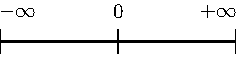
\includegraphics{figs/ns.pdf}
\end{center}
\caption{Number Axis}
\end{figure}

Each point on this axis represents a number. It may be integer or fractional
number. An integer is a whole number like -1, -2, 0, 5, 7 etc. Floating-point
numbers have fractional parts like 1.234. The important fact to note is that
between any two points there exists infinite numbers. In other words between
any two numbers there exists infinite numbers. For example, between 1.2 and 1.3
there are 1.21, 1.22, 1.23..., 1.29. Moreover between 1.21 and 1.22 there are
1.211, 1.212, 1.213 and so on. It enables us to represent a point on this
axis. The numbers I have written are supposedly in decimal number system. Base
of decimal number system is 10. Why because it consists of 10 distinct symbols
0 through 9. Similarly we can have any other number system. Popular number
systems in computers are binary, octal and hexadecimal not to mention decimal
ofcourse.

A number in a generic number system is given below:
\begin{equation}
(.. c_mb^{m-1} + c_{m-1}b^{m-2}+ ... + c_2b^1 + c1_b^0 + c_{-1}b^{-1} +
... + c_{-m}b^{-m} ) \\ = (... c_mc_{m-1}...c_2c_1.c_{-1}...c_{-m})_b
\end{equation}

All the terms with $c$  are called digits. The leftmost or leading digit is
called \textit{most significant digit} and the rightmost or trailing digit is
called \textit{least significant digit}. The . is called a point which
separates the integral part which is toards its left from the fractional part
which is towards its right. $b$  is known as radix or base of the number
system. Note that all digits will be between $0$ to $b-1$. So in our decimal
system $b$  is 10 therefore we have digits from 0 to 9. In binary number system
it is 2 therefore digits permitted are 0 and 1.

\subsection{Binary Number System}
As the name suggests binary number system has base of 2. Therefore it has only
two symbols. 0 and 1. This is the most popular system for computers becasue TTL
NAND and NOR gates which are the most basic logic gates using which other gates
are implemented in processor has only two voltage output levels because of
their operation in cut-off and saturation zones. These terms are better
understood with the help of a book on electronics which is out of scope of this
book. All binary numbers consist of 0 and 1. So the count is like 0, 1, 10, 11,
100, 101, 110, 111, 1000 and so on.

\subsubsection{Conversion of Unsigned Decimals and Bianries}
Consider a decimal number. Let us say 53 then how would be convert it to
binary. The technique is that of division. Please examine following carefully:

\hspace*{2cm}
\begin{Verbatim}[frame=single]
  2 | 53 | 1
  ----------
  2 | 26 | 0
  ----------
  2 | 13 | 1
  ----------
  2 | 6  | 0
  ----------
  2 | 3  | 1
  ----------
    | 1  |
\end{Verbatim}

So the binary is $110101_2$. First we divide 53 by 2 and write the
remainder. Then quotient is 26. We repeat the process for 26 therefore
remainder is 0 and quotient is 13. This we go on repeating till we have 1 as
quotient. Note that all the remainders will be 0 or 1 because divisor is
2. Similarly, final quotient is always 1. Now we take final quotient and start
writing remainders from top to bottom.

To convert binary to decimal let us examine following:

$1*2^5 +1*2^4 +0*2^3 +1*2^2 +0*2^1 +1*2^0 =53_{10}$

The power is to 2 because 2 is the base of source. It starts from 0 for unit's
position and increases to 1 and 2 for ten's and hundred's position and so
on. 1's and 0's are the values of that place. If you note carefully powers of 2
grow like 1, 2, 4, 8, 16, 32, 64, 128 and so on. Any number can be written by
using these powers at most one time. For example consider 100. I know it is
less than 128 so I will use 64. Then 36 remains. So I will use 32 and then
4. This means 100=64+32+4  which means power 6, 5 and 2 have been
used. Therefore, I can quickly write down number as $1100100_2$.

\label{fractional binary numbers}
Fractional numbers are slightly more complicated. Let us consider $1.1_2$  . In
decimal it will be $1+\frac{1}{2}$. This is 1.5 in decimal. Note that when you
convert a fractional part of binary to decimal denominator will always be power
of 2. For that matter when you convert from any base to decimal denominator
will be powers of that base. \textbf{Important:} Therefore, when you convert
from decimal to some base n then denominator of that decimal number can have
only those prime factors which are available in the set of prime factors of
$n$.

Let us say we have a fractional number in decimal .59 then to convert it to
decimal we multiply it with 2 which yields 1.018 which is greater than 1 so our
equivalent binary number is .1. Now we subtract 1 from 1.18 to get .18 which
is less than 1 so we multiply it with 2 again to get .36. Now since this is
less than 1 our equivalent binary number is .10. Repeating the process we get
.72 and .100 then 1.44 and .1001. We put 1 in binary part because decimal part
has become greater than 1. Now again we subtract 1 from decimal part to get .44
and repeat the process.

Operations such as addition, subtraction, multiplication and division are
similar in all number systems.

\subsection{2's Complement and 1's Complement}
2's complement and 1's complement are used to convert binary numbers to decimal
values. In 1's complement the number is obtained by inverting bits i.e. making
0 bit to 1 bit and 1 bit to 0 bit of the binary number in question.

Consider the following table which contains some numbers for 1's complement
of some 8-bit numbers.

The 2's complement of an $N$-bit number is defined as the complement with
respect to $2^N$; i.e. it is the result of subtracting the number
from $2^N$, which in binary is one followed by $N$ zeroes. This is also
equivalent to taking the 1's complement and then adding one, since the sum of
a number and its 1's complement is all 1 bits.



\begin{table}[H]
 \begin{center}
 \caption{8-bit 1's complement integers}
\begin{tabular}{|c|r|r|}
\hline
\textbf{Bits}&\textbf{Unsigned Value}&\textbf{1's Complement Value}\\
\hline
0111 1111&127&127\\
\hline
0111 1110&126&126\\
\hline
0000 0010&2&2\\
\hline
0000 0001&1&1\\
\hline
0000 0000&0&0\\
\hline
1111 1111&255&-0\\
\hline
1111 1110&254&-1\\
\hline
1000 0010&130&-125\\
\hline
1000 0001&129&-126\\
\hline
1000 0000&128&-127\\
\hline
\end{tabular}
\end{center}
\end{table}

For signed numbers MSB(most significant bit) decides sign in both 1's
complement as well as 2's complement. 1's complement has two zeroes. Positive
and negative. As you see in table that 1111 1111 is -0 because MSB is 1 so it
is a negative number and then if you invert all remaining bits then it turns
out to be 0. In a 1's complement system negative numbers are represented by the
arithmetic negative of the value. An $N$-bit 1's complement number system can
represent integres in the range $-2^{N-1} - 1$ to $-2^{N-1} - 1$.

Now it is easy to do addition, subtraction, multiplication, division and other
arithmetic operations. Subtraction for 1's complement is a bit
different. Consider the following:

\begin{Verbatim}[frame=single]
    0000 0110      6
  - 0001 0011     19
    ===========   ====
    1 1111 0011    −12    -An end-around borrow is produced, and the sign bit
                          of the intermediate result is 1.
  - 0000 0001        1   -Subtract the end-around borrow from the result.
    ===========   ====
    1111 0010      −13    -The correct result (6 - 19 = -13)
\end{Verbatim}

Borrows are propagated to the left. If the borrow extends past the end then it
is said to have ``wrapped around'', a condition called an ``end-around
borrow''. When this occurs, the bit must be subtracted from the right-most bit
or least significant bit(LSB). This does not occur in 2's complement arithmetic.

As you see in table and also you can verify the value becomes negative if its
1's complement is computed. However, 2's complement is used on most of
computers because of two zeroes in 1's complement, borrowing being complicated
etc. 

Consider following table of 2's complement 3-bit binary numbers:

\begin{table}[H]
  \begin{center}
    \caption{3-bit 2's complement integers}
    \begin{tabular}{|c|r|r|}
      \hline
      \textbf{Bits}&\textbf{Unsigned value}&\textbf{2's complement value}\\
      \hline
      011&3&3\\
      \hline
      010&2&2\\
      \hline
      001&1&1\\
      \hline
      000&0&0\\
      \hline
      111&7&-1\\
      \hline
      110&6&-2\\
      \hline
      101&5&-3\\
      \hline
      100&4&-4\\
      \hline
    \end{tabular}
  \end{center}
\end{table}

Clearly, since $N$-bit 1's complement can represent numbers in range
$-2^{N-1}-1$ to $2^{N-1} + 1$ 2's complement of $N$-bit can represent
$-2^{N-1}$ to $2^{N-1} - 1$ as it does not have negative 0 i.e. its range is
more by 1 number.

The 2' complement system has the advantage that operations of addition,
subtraction, and multiplication are same as unsigned binary numbers (as long as
the inputs are represented in the same number of bits and any overflow beyond
those bits is discarded from the result). This property makes the system both
simpler to implement and capable of easily handling higher precision
arithmetic. Also, as mentioned above zero has only a single 
representation, avioding the subtleties associated with negative zero, which
exists in 1's complement systems.

The value $v$ of an $N$-bit integer $b_{N-1} b_{N-2} \dots b_0 $is given by the
following formula:

\begin{equation}
v=-b_{N-1} 2^{N-1} + \sum_{i=0}^{N-2} b_i 2^i
\end{equation}

I will leave it up to you, the reader, to perform basic operations like
addition, subtraction, multiplication, division etc.

Now we can proceed to discuss technical details of C programming
language. There are certain rules in every language, certain grammar which
dictates the
way language will be spoken and written. It has a script to write
using. Similarly, programming languages have BNF (Backus-Naur Form)
context-free grammar. There are valid characters in a programming language and
a set of keywords. There are constructs to handle control flow, loops
etc. There are facilities provided by language to deal with numbers and strings
separately, to reuse the code and some basic data structures to facilitate
programming. However, programming language ruleset is very small compared
to a natural programming language. Also, when using natural programming
language like talking to someone or writing something the other person can
understand your intent but in programming you cannot violate rules. The grammar
is context-free. Compilers or interpreters cannot deduce your intent by reading
code. They are not intelligent. You make a mistake and it will refuse to listen
to you no matter what you do. Therefore, it is very essential to understand
these rules very clearly and correctly.

Note that C language is govered by ISO specification \textbf{ISO/IEC
  9899:2011}. As much as I would like to refer to specification there are
financial reasons why I will not because it is expensive and I do not expect
all of readers to buy this. Therefore, I will be referring to final draft
version which you can download from
\url{http://www.open-std.org/jtc1/sc22/wg14/www/docs/n1570.pdf}. It will be
almost same as final revision and costs nothing. Sections of this document will
be referred like \S(section number).

\section{The C Character Set}
The following form the C character set you are allowed to use in it which is
given in \S(5.2.1):

\begin{Verbatim}[frame=single]
[a-z] [A-Z] [0-9] ~ ! # % ^ & * ( ) - = [ ] \ ; ' , . / _ + { } | : " < > ?
\end{Verbatim}
\index{character set}

This means along with other symbols you can use all English alphabets (both
uppercase and lowercase) and Arabic numerals. Symbols like \texttt{\$} and
\texttt{@} are not part of C's character set. But strings can contain any
these characters also. Strings are sequence of characters with double quotes
and double quotes iteself are escaped with \texttt{$\backslash$}. Also,
\texttt{\$} and \texttt{@} can also be value of characters. Characters are
values containing single characters withing single quotes. We will see more of
these in their individual sections. However, English is not the only
spoken language in the world. Therefore in other non-English speaking counties
there are keyboard where certain characters present in above set are not
present. The inventors of C were wise enough to envision this and provide the
facility in form of trigraph sequences. Given below is the trigraph sequence
table given in \S(5.2.1.1):

\begin{table}[H]
 \begin{center}
 \caption{Trigraph Sequences}
\begin{tabular}{|c|c|c|c|c|c|}
\hline
\textbf{Trigraph}&\textbf{Equivalent}&\textbf{Trigraph}&\textbf{Equivalent}&\textbf{Trigraph}&\textbf{Equivalent}\\
\hline
??=&\#&??'&\textasciicircum&??!&|\\
\hline
??(&[&??)&]&??$<$&\{\\
\hline
??$>$&\}&??/&\textbackslash&??-&\textasciitilde\\
\hline
\end{tabular}
\end{center}
\end{table}
\index{trigraph sequences}

However, you should refrain from using trigraph sequences for portability 
reasons as suggested by GNU coding standards.

\section{Keywords}
The following given in \S(6.4.1) are reserved keywords for C programming language which you are not 
allows to use other than what they are meant for:
\index{keywords}
\begin{table}[H]
 \begin{center}
  \caption{Keywords of C}
  \begin{tabular}{l l l l l}
    auto & break & case & char & const\\
    continue & default & do & double & else\\
    enum & extern & float & for & goto\\
    if & inline & int & long & register\\
    restrict & return & short & signed & sizeof\\
    static & struct & switch & typedef  & union\\
    unsigned & void & volatile & while & \_Alignas\\
    \_Alignof& \_Atomic & \_Bool & \_Complex & \_Generic \\
    \_Imaginary & \_Noreturn & \_Static\_assert & \_Thread\_local\\
  \end{tabular}
 \end{center}
\end{table}

These keywords are special in C as said and cannot be used for variable names 
or funciton names or otherwise other than in strings and comments.

\section{Identifiers}
The names which we give to our variables are known as identifiers
\S(6.4.2). Please read this section carefully and make sure understand
the rules for naming identifiers. Later at the end of chapter there are some
simple problems to practice with.

Identifoers are something  with which we identify the variables or constants or
functions etc. In other words
since memory locations are difficult to remember for us, human beings, we
assign these memory locations more meaningful names in form of identifiers. As
you have already seen what is allowed  in C's character set but not all are
allowed in an identifiers name. Only alphabets from English language both
lowercase and uppercase(they are distinct),
Arabic digits from zero to nine and underscore (\_) are allowed in an
identifiers name. The rule for constructing names is that among the allowed
characters it can only begin with only English alphabets and
underscore. Numbers must not be first character. For example, \texttt{x,
  \_myVar, varX} and \texttt{yourId78} are all valid names. However, take care
with names starting from underscore as they are mostly used by different
library authors. Invalid identifier examples are \texttt{9x, my\$} and
\texttt{your age}. If the identifier name contains extended
characters(i.e. other than what is mentioned for simplicity like, chinese,
european, japanese etc) then it will be replaced with an encoding of universal
character set, however, it cannot be first chgaracter.

Length of an identifer for 31 characters, as specified in \S(5.2.4.1), is
guaranteed across all platforms.

\section{Programming}
Let us revisit our first program and try to understand what it does. Here I am 
giving code once again for quick reference:

\begin{Verbatim}[frame=single]
// My first program
/* Description: This program does nothing.*/

#include <stdio.h>

int main(int argc, char* argv[])
{
  return 0;
}
\end{Verbatim}

You can now issue a command as \texttt{\$gcc nothing.c} where 
\texttt{nothing.c} is the filename by which you saved the source code. Note 
that \texttt{\$} is the prompt not part of command itself. Then you can do an 
ls and you will find that \texttt{a.out} is a file which has been produced by 
gcc. Now you can run this program by saying \texttt{\$./a.out} and nothing 
will happen. But if you type \texttt{\$echo \$?} then you will find that 0 is 
printed on screen which is nothing but 0 after \texttt{return} of our program.

As you can see this program does almost nothing but it is fairly complete 
program and we can learn a lot from it about C. Let us try to dissect it line
by line. The first line is a comment. 
Whenever C compiler parses C programs and it encounters \texttt{//} it ignores 
rest of line as code i.e. it does not compile them. This type of single line 
comment were introduced in C99 standard and if your compiler is really old the 
compiler may give you error message about it. The second line is
also comments. Anything between \texttt{/*} and \texttt{*/} is ignored like 
\texttt{//}. However, be careful of something like \texttt{/* some comment */
  more comment */}. Such comments will produce error messages and your program
will fail to compile. The reason for this is when first \texttt{*/} is
encountered by parser or compiler it will complete its token for the comment
and then further portion which we intented to be part of comment will cause
syntax error. 

Comments are very integral part of programming. They are used to describe 
various things. You can write whatever you want. They may also be used to 
generate documentation with tools like doxygen. Typically comments should tell
what the program is doing not how. Sometimes how can be covered, when the logic
is really complex. One should be generous while commenting the code.

The next line is \texttt{\#include <stdio.h>}. \texttt{\#include} is a
preprocessor directive. The preprocessor directive is handled by the C
preprocesor which is handled by C preprocessor which looks in four directories
for include files. The include filename comes after \texttt{\#include} either in
angular brackets or double quotes. The C preprocessor looks for these at four
different places at least out of which one or posiibly two is of interest for
now as we are dealing with angular brackets. Depending on the way your compiler
is installed the file \texttt{stdio.h} may be in \texttt{/usr/include} or
\texttt{/usr/local/include} but then again it may be in a non-standard path
also although possibility of that is very less and then it is controlled by
parameters whose discussion is beyond the scope of book. Let us say
\texttt{stdio.h} is present in either of aforementioned directories then the C
preprocessor will copies the contents and pastes them in source file along the
way putting \texttt{\#line} macros which are used for debugging
purposes. \texttt{\#line} macro is discussed later in the chapter which deals
with macros. You can see the output of C preprocessor by typing \texttt{\$gcc
  -E nothing.c} since it will scroll a lot on you terminal you can use a pager
like \texttt{less} to read it. The \texttt{-E} tells \texttt{gcc} to just allow
preprocessoing and not compile and link the file.

Next line is \texttt{int main(int argc, char* argv[])}. Now this is very special
function. Every complete executable(shared objects or dlls or archive
libraririe do not have main even though they are C programs) C program will
have one main function unless you do assembly hacking. This function is where
the programs start. The first word \texttt{int} is a keyword which shirthand
for integer. This signifies the return type of function. \texttt{main} is the
name of the function. Inside parenthesis you see \texttt{int argc} which tells
how many arguments were passed to program and is short form of argument
count. While \texttt{char* argv[]} is a pointer to array which we will see
later. For now let us just remember that it holds all the arguments to the
program including the program name.

Next is a brace. The scope in C is determined by braces. Something outside any
brace has global scope (we will see these later), something inside first level
of brace has function or local scope. Something inside second or more level of
braces have got that particular block scope. Scope here means that when there
will be a closing brace that particular variable which is valid in that scope
will cease to exist. However, we do not have to worry about that yet as we do
not have any variable. Just note that a corresponding closing brace will be the
end of main function. For every opening brace which starts a scope a closing
brace is mandatory.

Next line is \texttt{return 0;} This means whoever has called \texttt{main()}
will get a 0 as \texttt{return} is returning 0. In this case, receiver is the
shell or operating system 
which has invoked the very program. The semicolon is called the terminator and
used also on Java or C++ for example. The very requirement of semicolon is to
terminate the statement and move on to next statement.

However, the program shown does not do much. Let us write a program which has
some more functionality and we can explore more of C. So here is a program
which takes two integers as input from users and presents their sum as
output. Here is the program:

\begin{Verbatim}[frame=single]
// My second program
// Author: Shiv S. Dayal
// Description: It adds two numbers

#include <stdio.h>

int main()
{
  int x=0, y=0, sum=0;

  printf("Please enter an integer:\n");
  scanf("%d", &x);

  printf("Please enter another integer:\n");
  scanf("%d", &y);

  sum = x + y;

  printf("%d + %d = %d\n", x, y, sum);

  return 0;
}
\end{Verbatim}
and the output is:
\begin{Verbatim}[frame=single]
shiv@shiv:~/book/code$ ./addition
Please enter an integer:
7
Please enter another integer:
8
7 + 8 = 15
shiv@shiv:~/book/code$
\end{Verbatim}

Note that \texttt{shiv@shiv:~/book/code\$} is the prompt.

Let us discuss new lines one by one. The line \texttt{int x=0, y=0, z=0;} is
declaration and definition or initialization of three ints. \texttt{int}
keyword in C is used to represent integers. Now we have three integers with
there values set to 0. Note that how the variables are separated by commas and
terminated by semicolon(as we saw in last program also). We could have also
written it like this:

\begin{Verbatim}[frame=single]
int x;
int y;
int z;

x = 0;
y = 0;
z = 0;
\end{Verbatim}

or

\begin{Verbatim}[frame=single]
int x, y, z;

x = y = z = 0;
\end{Verbatim}

However, the first method is best and most preferred as it prevents use before
definition. \texttt{int} is a data-type in C. \texttt{x, y,} and \texttt{z} are
called variables of type \texttt{int}. This means that the size of these
variables will be same as \texttt{int}. Note that 
C is a statically typed language and all types have predefined memory
requirements. In cour case, \texttt{int} requires 4 bytes on 32-bit and 64-bit
systems but 2 bytes on 16-bit systems.

Let us learn a bit about \texttt{printf}. This function is declared in
stdio.h. The prototype of \texttt{printf()} is

\begin{Verbatim}[frame=single]
int printf(const char *restrict format, ...);
\end{Verbatim}

The first argument format is what we have in first two function calls. The
second is a \texttt{...} which means it can take variable number of arguments
known as variable-list. We have seen this in the third call.This means it will
take a string with optional variable no. of arguments. The string is called the
format-string and determines what can be printed with supplied arguments. These
\texttt{...} are used to supply variable no. of arguments. In the first two
\texttt{printf()} statements we just print the format-string so that is
simple. However, in the last one, we have format as \texttt{\%d} which
signifies a decimal integer. The integers printed are in the same order in
which they were supplied.

\texttt{scanf()} is scan function which scans for keyboard input. As by now you
know that \texttt{\%d} is for decimal integer but we have not said \texttt{x}
or \texttt{y}. The reason is \texttt{x} and \texttt{y} are names for memory
addresses while
\texttt{\&x} and \texttt{\&y} are the addresses of \texttt{x} and \texttt{y} in
memory. \texttt{scanf()} needs the memory address to which it can write the
contents to. You will see \texttt{\&} operator in action later when we deal
with pointers. Just remember for now that to use a simple variable with
\texttt{scanf()} requires \texttt{\&} before its name.

Till now we have just seen only \texttt{int} data-type but then there are more
data types for other types of numbers, characters and strings. Let us see them
one by one.

\section{Data Types}
What are data types? Why C needs data types? C is a statically typed language
that is every variable has a type associated with it. Types are discussed in
specification in great length in \S(6.2.5) to \S(6.2.8).
These types determine
what kind of values these variables can hold and how they will be interpreted.
Say we encode
character `A' for 10101 will it be easy for you to see A or numbers. Also,
numbers range from $-\infty$ to $\infty$. Also, since C is statically typed the
sizes of data types have to be known at compile time. Because the data type is
known a compiler can detect whether we are storing corect type of values in
corect type of variables at compilation time. Also, it allows compiler to do
certain optimization which efffects the runtime performance of the program
during execution. There are four types of
data types. Integral, floating-point, arrays and pointers. Here, I will deal
with the two former types and leave latter two for later. The integral types
are \texttt{char, short int, int, long} and \texttt{long long} and
floating-point types are \texttt{float, double} and \texttt{long
  double}. \texttt{signed} and \texttt{unsigned} are sign modifiers which also
modified the range of data types but do not affect their memory
requirements. By default all basic data types are \texttt{signed} in nature and
you must qualify you variables with \texttt{unsigned} if you want that
behavior. \texttt{short} and \texttt{long} are modifiers for size which the
data type occupies but I consider them as different types because memory
requirements are different. The ranges of integral data types directly reflect
their memory requirements and if you know how much memory they are going to
occupy you can easily compute their ranges. The range of floating-point comes
from IEEE specification. IEEE standard document 754 governs the binary
representation of floating point numbers which you can read at
\url{http://www.eecs.berkeley.edu/~wkahan/ieee754status/IEEE754.PDF}. You can
also buy it from IEEE's website. I will describe it later.

Let us write a program to find out ranges for integral data types:

\begin{Verbatim}[frame=single]
// Description: It gives ranges of integral data types

#include <stdio.h>
#include <limits.h>

int main()
{
  printf("Size of char is..........%d\n", sizeof(char));
  printf("Size of short int is.....%d\n", sizeof(short int));
  printf("Size of int is...........%d\n", sizeof(int));
  printf("Size of long is..........%d\n", sizeof(long));
  printf("Size of long long is.....%d\n", sizeof(long long));
  printf("Size of float is.........%d\n", sizeof(float));
  printf("Size of double is........%d\n", sizeof(double));
  printf("Size of long double is...%d\n", sizeof(long double));c

  return 0;
}
\end{Verbatim}

Here \texttt{sizeof} is a compile time operator which computes size of any type
passed to it as an argument. So it is computing sizes of all the data types as
shown in the program. The output is given below:

\begin{Verbatim}[frame=single]
Size of char is..........1
Size of short int is.....2
Size of int is...........4
Size of long is..........8
Size of long long is.....8
Size of float is.........4
Size of double is........8
Size of long double is...16
\end{Verbatim}

Please note that the output shown is on 64-bit machine and it will be different
on 32-bit machines.

\section{Integers}
Integers are probably simplest to understand of all data types in C so I am
discussing them before any other type. As you have seen the keyword for
declaring integer type is \texttt{int}. An integer can be 2 bytes or 4 bytes. A
16-bit compiler will have integer of 2 bytes while a 32-bit or 64-bit compiler
will have a 4 byte integer. The specified minimum size of an integer is 2
bytes. Since most modern computers are either 32-bit with
64-bit becoming more dominant we will assume in this book that integer's size
is 4 bytes or 32-bit implicitly because 32-bit \texttt{gcc} gives a 32-bit
integer. There is a keyword \texttt{signed} which when 
applied to a data type splits the range into two parts. Since interger is 32
bit so it will be split in the range from $-2^{31}$ to $2^{31} - 1$. By default
integers, characters and long are \texttt{signed}. Floats and doubles are
always \texttt{unsigned} and have no signed counterpart. When the integer will
be \texttt{unsigned} then the positive range doubles and it becomes $0$ to
$2^{32} - 1$. When the value of intger is more than its range then the values
rotate in the using modulus with the largest value of the range which is also
known as \texttt{INT\_MAX} or \texttt{INT\_MIN}. For \texttt{unsigned} types it
is \texttt{UINT\_MAX}. These are macros and are defined in \texttt{limits.h}
which you can find in \texttt{/usr/include} or \texttt{/usr/local/include} by
default.

There are four different types of integers based on their storage
reuirement. \texttt{short int, int, long,} and \texttt{long long.} Short
integers are always two bytes. Signed short integer has a range of -32768 to
32767 while unsigned of that has a range of 0 to 65535. Plain integers
i.e. \texttt{int} has already been discussed. \texttt{long} are having a
minimum storage reuirement of 4 bytes. Usually it is large enough to represent
all memory addresses of the system because \texttt{size\_t} is
\texttt{unsigned long.}

\section{Characters}
A \texttt{char} is 1 byte i.e. 8 bits or \texttt{CHAR\_BIT} bits. So its signed
version i.e. 2's 
complement where half the range is negative and half is positive will have
value from -128 to 127. Well that is not exactly opposite because we have only
one zero for positive and negative numbers. If it would have been 1's
complement then range would have been from -127 to 127 but since computers
follow 2's complement the specification clearly mentions that range should be
from $-2^7$ to $2^7 - 1.$ Note that chars are fundamentally integral types and
ascii symbols are first 128 numbers or in other words they are 7-bit numbers.

So a character `0' is internally 48 in decimal which is its integral or
internally it is handled as a sequence of binary numbers representing
\texttt{0x30} in hexdecimal. These integral values for characters are known as
ASCII value. A full table of ASCII values is given in the appendix A.

A simple program which takes input for few characters and then prints them on
console along with their ascii values is given below:

\begin{Verbatim}[frame=single]
#include <stdio.h>

int main()
{
  char c = 0;
  char c1 = 0, c2 = 0;

  printf("Enter a character on your keyboard and then press ENTER:\n");
  scanf("%c", &c);
  printf("The character entered is %c and its ASCII value is %d.\n", c, c);
  // Their remains '\n' in the stdin stream which needs to be cleared.
  getchar();
  printf("Enter a pair of characters on your keyboard and then press \
ENTER:\n");
  scanf("%c%c", &c1, &c2);
  printf("The characters entered are %c and %c and their ASCII \
values are %d and %d respectively.\n", c1, c2, c1, c2);

  short int si = 0;

  si = c1 + c2;

  printf("The sum of c1 and c2 as integers is %hd.\n", si);

  return 0;
}
\end{Verbatim}

A sample run may have following output:

\begin{Verbatim}[frame=single]
Enter a character on your keyboard and then press ENTER:
1
The character entered is 1 and its ASCII value is 49.
Enter a pair of characters on your keyboard and then press ENTER:
12
The characters entered are 1 and 2 and their ASCII values are 49 and 50
respectively.
The sum of c1 and c2 as integers is 99.
\end{Verbatim}

As you can see from the program that characters are internally stored as
integers and we can even perform integers which we normally perform on
numbers like addition as shown. We can perform other operation as subtraction,
multiplication and division, however, most of the time addition or subtraction
only makes sense to advance the characters in their class. Multiplication and
division of characters with other characters or integers does not make sense.

One problem of concern is the extra \texttt{\textbackslash n} in the input
stream. It does not cause trouble with integers but when you want to read
characters then the \texttt{Enter} or \texttt{Return} keys which may be left
over from the last input will cause trouble. \texttt{\textbackslash n} is
recognized as a character and will be assigned to next variable if it is in
\texttt{stdin.} One of the ways to remove it is to make a call to
\texttt{getchar} which reads one character from the \texttt{stdin} stream.

\section{Sizes of Integer Types}
Before going any further and discussing floats and doubles let us take a look
at limits of various integral type as specified in specification. Note that the
output from your compiler may be larger but not smaller because these are
minimum values. The limits given below and the limits which will be given for
floating point numbers are described in \texttt{<limits.h>} and
\texttt{<float.h>}.

\begin{itemize}
\item[---] number of bits for smallest object that is not a bit-field (byte)\\
\texttt{CHAR\_BIT}\hfil\hspace*{2cm}\texttt{8}
\item[---] minimum value for an object of type \texttt{signed char}\\
\texttt{SCHAR\_MIN}\hfil\hspace*{2cm}\texttt{-127 //} $-(2^7 - 1)$
\item[---] maximum value for an object of type \texttt{signed char}\\
\texttt{SCHAR\_MAX}\hfil\hspace*{2cm}\texttt{+127 //} $2^7 - 1$
\item[---] maximum value for an object of type \texttt{unsigned char}\\
\texttt{UCHAR\_MAX}\hfil\hspace*{2cm}\texttt{255 //} $2^8 - 1$
\item[---] minimum value for an object of type \texttt{char}\\
\texttt{CHAR\_MIN}\hfil\hspace*{2cm}\textit{see below}
\item[---] maximum value for an object of type \texttt{char}\\
\texttt{CHAR\_MAX}\hfil\hspace*{2cm}\textit{see below}
\item[---] maximum number of bytes in a multibyte character, for any supported
  locale\\
\texttt{MB\_LEN\_MAX}\hfil\hspace*{2cm}\texttt{1}
\item[---] minimum value for an object of type \texttt{short int}\\
\texttt{SHRT\_MIN}\hfil\hspace*{2cm}\texttt{-32767 //} $-(2^{15} - 1)$
\item[---] maximum value for an object of type \texttt{short int}\\
\texttt{SHRT\_MAX}\hfil\hspace*{2cm}\texttt{+32767 //} $2^{15} - 1$
\item[---] maximum value for an object of type \texttt{unsigned short int}\\
\texttt{USHRT\_MAX}\hfil\hspace*{2cm}\texttt{65535 //} $2^{16} - 1$
\item[---] minimum value for an object of type \texttt{int}\\
\texttt{INT\_MIN}\hfil\hspace*{2cm}\texttt{-32767 //} $-(2^{15} - 1)$
\item[---] maximum value for an object of type \texttt{int}\\
\texttt{INT\_MAX}\hfil\hspace*{2cm}\texttt{+32767 //} $2^{15} - 1$
\item[---] maximum value for an object of type \texttt{unsigned int}\\
\texttt{UINT\_MAX}\hfil\hspace*{2cm}\texttt{65535 //} $2^{16} - 1$
\item[---] minimum value for an object of type \texttt{long int}\\
\texttt{LONG\_MIN}\hfil\hspace*{2cm}\texttt{-2147483647 //} $-(2^{31} - 1)$
\item[---] maximum value for an object of type \texttt{long int}\\
\texttt{LONG\_MAX}\hfil\hspace*{2cm}\texttt{+2147483647 //} $2^{31} - 1$
\item[---] maximum value for an object of type \texttt{unsigned long int}\\
\texttt{ULONG\_MAX}\hfil\hspace*{2cm}\texttt{4294967295 //} $2^{32} - 1$
\item[---] minimum value for an object of type \texttt{long long int}\\
\texttt{LLONG\_MIN}\hfil\hspace*{2cm}\texttt{-9223372036854775807 //} $-(2^{63} - 1)$
\item[---] maximum value for an object of type \texttt{long long int}\\
\texttt{LLONG\_MAX}\hfil\hspace*{2cm}\texttt{+9223372036854775807 //} $2^{63} - 1$
\item[---] maximum value for an object of type \texttt{unsigned long long int}\\
\texttt{ULLONG\_MAX}\hfil\hspace*{2cm}\texttt{18446744073709551615 //} $2^{64} - 1$
\end{itemize}

If the value of an object of type \texttt{char} is treated as a signed integer
when used in an expression, the value of \texttt{CHAR\_MIN} shall be the same
as that of \texttt{SCHAR\_MIN} and the value of \texttt{CHAR\_MAX} shall be the
same as that of \texttt{SCHAR\_MAX}. Otherwise, the value of \texttt{CHAR\_MIN}
shall be 0 and the value of \texttt{CHAR\_MAX} shall be the same as that of 
\texttt{UCHAR\_MAX}. The value \texttt{UCHAR\_MAX} shall equal $2^{CHAR\_BIT} -
1$.

Values given above have the form of 1's complement in which positive zero and
negative zero are treated differently while computers in general work using 2's
complement so you will notice that the minimum values are extended by 1. So for
example, \texttt{SHRT\_MIN} in \texttt{<limits.h>} is given as -32768 and so
are all minimum values.

\section{Floating Types}
Floating point representation is a lot more complicated in computers than it
is for us human beings. C specification takes floating points description and
specification from IEC 60559:1989 which is a standard for floating point
arithmetic whihc is same as IEEE 754. In C there are three types of flaoting
point numbers \texttt{float, double} and \texttt{long double.} It is describved
in specification in \S(5.2.4.2.2).

A floating-point number is used to represent real-world fractional value which
is a trade-off between range and accuracy because as I said in \ref{fractional
  binary numbers}, a decimal fraction cannot represented in binary unless the
denominator of that number is an integral power of 2. A number is, in general,
represented approximately to a fixed number of significant digits (the
significand) and scaled using an exponent; numbers are usually binary, octal,
decimal or hexadecimal. A number that can be represented exactly is of the
following form:

$$\text{significand} \times \text{base}^\text{exponent}$$

For example, $1.2345 = \underbrace{12345}_\text{significand} \times
\,\underbrace{10}_\text{base}\!\!\!\!\!\!^{\overbrace{-4}^\text{exponent}}$

The term floating point refers to the fact that a number's radix point (decimal
point, or, more commonly in computers, binary point) can ``float''; that is, it
can be placed anywhere relative to the significant digits of the number.

\subsection{Representation of Floating-Point Numbers}
Given below are pictorial representations of 32-bit and 64-bit floating point
numbers:
\begin{figure}[H]
\begin{center}
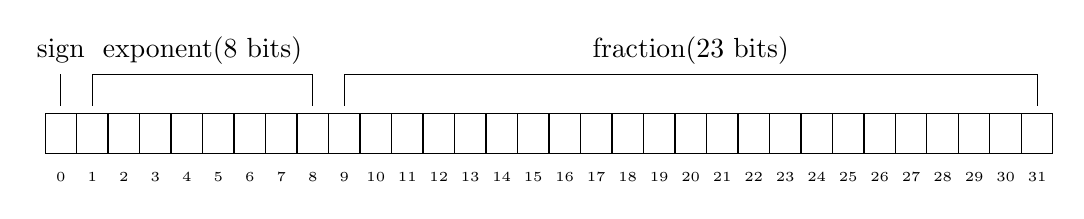
\begin{tikzpicture}[node distance=1.8cm]
  \foreach \x in {0, ..., 31}
  \draw (\x*0.4cm, 0) -- +(.4cm, 0) -- +(.4cm, 0.5cm) -- +(0, .5cm) --
  cycle;
  \draw (0.2cm, 0.6cm) -- (0.2cm, 1cm);
  \draw (0.6cm, 0.6cm) -- (0.6cm, 1cm) -- (3.4cm, 1cm) -- (3.4cm, 0.6cm);
  \draw (3.8cm, 0.6cm) -- (3.8cm, 1cm) -- (12.6cm, 1cm) -- (12.6cm, 0.6cm);
  \foreach \x in {31, ..., 0}
  \node at (\x*0.4cm, 0) [xshift=.2cm, yshift=-.3cm, align=center] {\tiny \x};
  \node at (0.2cm, 1.3cm) [align=center] {sign};
  \node at (2cm, 1.3cm) [align=center] {exponent(8 bits)};
  \node at (8.2cm, 1.3cm) [align=center] {fraction(23 bits)};
\end{tikzpicture}
\caption{32-bit floating-point numbers}
\label{fig:32-bit floating point numbers}
\end{center}
\end{figure}

Similarly in 64-bit floating point numbers we have 1 bit for sign, 11 bits for
exponent and 52 bits for fractional part. Clearly zero will be represented by
all sign and exponent bits having value 0 for them.

C also has concept of positive and negative infinities. Sign bit is 0 for
positive infinity and 1 for negative infinity. Fractional bits are 1 while
exponent bits are all 1.

Certain operations cause floating point exceptions like division from zero or
square rooting a negative number. Such exceptions are represented by NANs which
stands for ``not a number''. Sign for NaNs is similar i.e. 0 for positive and 1
for negative. Exponent bits are 1 and fractional part is anything but all 0s
because that represents positive infinity.

There is also four rounding modes which we will see later.

Now let us see a program to see how we can take input and print the floating
point numbers.

\begin{Verbatim}[frame=single]
#include <stdio.h>

int main()
{
  float f = 0.0;
  double d = 0.0;
  long double ld = 0.0;

  printf("Enter a float, double and long double separated by space:\n");
  scanf("%f %lf %Lf", &f, &d, &ld);

  printf("You entered %f %lf %Lf\n", f, d, ld);

  return 0;
}
\end{Verbatim}

If you run this you might have following output:

\begin{Verbatim}[frame=single]
Enter a float, double and long double separated by space:
3.4 5.6 7.8
You entered 3.400000 5.600000 7.800000
\end{Verbatim}

By default these print upto six significant digits but doubles have double
precision as we have studied. Now that we know basic types let us learn a bit
about input/output.

\section{Boolean Data Type}
A boolean type has only two values possible; \texttt{true} and
\texttt{false}. Fundamentally a boolean is an integer. 0 is considered as
\texttt{false} while all other are treated as \texttt{true} including negative
integers. \texttt{true} and \texttt{false} are macros (which we will see later)
which are defined in \texttt{<stdbool.h>} and they expand to 1 and 0
respectively. The type \texttt{bool} is a macro which expands to
\texttt{\_Bool}. Let us see a small program with bolleans:

\begin{Verbatim}[frame=single]
#include <stdio.h>
#include <stdbool.h>

int main()
{
  bool bcpp      = 4;
  _Bool bc       = 5;
  bool True      = true;
  _Bool False    = false;
  bool bFalseCPP = -4;
  _Bool bFalseC  = -7;

  printf("%d %d %d %d %d %d\n", bcpp, bc, True, False, bFalseCPP, bFalseC);

  return 0;
}
\end{Verbatim}

and the output is:

\begin{Verbatim}[frame=single]
1 1 1 0 1 1
\end{Verbatim}

Note that \texttt{true} and \texttt{false} are keywords while \texttt{True} and
\texttt{False} are identifiers.

\section{Complex Type}
C99 introduced another type \texttt{complex}. As you may know a complex has two
parts real and imaginary. These parts of a complex individually are
floating-point numbers i.e. they can be represented by \texttt{float, double}
or \texttt{long double}. The header \texttt{<complex.h>} deals with complex
numbers and there are lots of useful functions to use and manipulate complex
numbers which are detailed in the reference. Let us see a simple example:

\begin{Verbatim}[frame=single]
#include <stdio.h>
#include <complex.h>

int main()
{
  double complex z = 4.0 + 3.0i;

  printf("Absolute value of z is %lf\n", cabs(z));

  double complex zConj = conj(z);
  printf("Imaghinary part of conjugate is now %lf\n", cimag(zConj));

  return 0;
}
\end{Verbatim}

Since we have used \texttt{<complex.h>} we need to link math library to compile
this program so the compilation command would look like \texttt{\$gcc -o complex
complex.c -lm}. The \texttt{-lm} part is mandatory for compilation of this
program. Let us see the output:

\begin{Verbatim}[frame=single]
Absolute value of z is 5.000000
Imaghinary part of conjugate is now -3.000000
\end{Verbatim}

I have shown only two functions \texttt{cabs} and \texttt{cimag} but there are
a lot more and very useful functions available to do computations on complex
numbers. The way to declare a complex number is shown. It is a combination of
real part and imaginary part where imaginary part is coupled with $i$ which is
given by $i = \sqrt{-1}$. Here, \texttt{cabs} computes absolute value of
complex number which is given by $\sqrt{x^2 + y^2}$ where complex number is
given by $x + iy$. We will see rest of the functions in reference.

\section{Void and Enum}
The \texttt{void} type comprises an empty set of values; it is an incomplete
object type\footnote{An incomplete type is a type whose size is unknown.} that
cannot be completed. You cannot declare variables with type void. You cannot
declare an array of\texttt{void} type. Any declaration which requires size of
type to be known cannot have \texttt{void} as its type. However, we can declare
pointers of type \texttt{void} because pointers do not require size of type to
be known. For this reason \texttt{void} pointers are used as generic pointers
and is used to convert one type of pointers into another. It is a low-level
type and should be used sparigly. We will see examples of \texttt{void} type
later in the book.

Enum type is an integral type and is used as symbolic constants. An enumeration
is is a set of integers(values). You can do all operations of an enum on an
enumeration member which you can do on an integer. It starts from zero by
default and increments by one unless specifically specified. Given below is an
example of \texttt{enum} type.

\begin{Verbatim}[frame=single]
#include <stdio.h>

int main()
{
  typedef enum {zero, one, two} enum1;
  typedef enum {alpha=-5, beta, gamma, theta=4, delta, omega} enum2;

  printf("zero = %d, one = %d, two=%d\n", zero, one, two);
  printf("alpha = %d, beta = %d, gamma=%d, theta=%d, delta=%d, omega=%d\n", \
          alpha, beta, gamma, theta, delta, omega);

  return 0;
}
\end{Verbatim}

and the output is

\begin{Verbatim}[frame=single]
zero = 0, one = 1, two=2
alpha = -5, beta = -4, gamma=-3, tehta=4, delta=5, omega=6
\end{Verbatim}

\section{Literals}
There are four categories of constants: character, integer, floating-point, and
enumeration constant. There are certain rules about constants. Commas and
spaces are not allowed except for character and string constants. Their range
cannot outgrow the range of there data type. For numeric type of stants they
can have a leading (-)minus sign.

Given below is an example of integer constants:

\begin{Verbatim}[frame=single]
#include <stdio.h>

int main()
{
  int decimal = 7;
  int octal = 06;
  int hex = 0xb;

  printf("%d %o %x\n", decimal, octal, hex);

  return 0;
}
\end{Verbatim}

and the output is:

\begin{Verbatim}[frame=single]
7 6 b
\end{Verbatim}

As you can see there are three different categories for integer constants:
decimal constants (base 10), octal constants (base 8) and hexadecimal constants
(base 16). Also, you must have noticed how a zero is prefixed before octal type
and a zero and x for hexadecimal type. The \texttt{\%d} format specifier is
already known to you for signed decimals. However, now you know two more
\texttt{\%o} and \texttt{\%x} for unsigned octal and unsigned hexadecimal
respectively. For unsigned integer it is \texttt{\%u}. There is one more format
specifier which you may encounter for signed decimal and that is
\texttt{\%i}. Note that there is nothing for binary constants.

A floating-point constant is a base-10 number that contains either decimal
point or exponent or both. Given below is an example of floating-point
constants:

\begin{Verbatim}[frame=single]
#include <stdio.h>

int main()
{
  float f = 7.5384589234;
  double d = 13.89457883453857823;
  long double ld = 759.8263478234729;

  printf("%f %lf %Lf\n", f, d, ld);

  return 0;
}
\end{Verbatim}

and the output is

\begin{Verbatim}[frame=single]
7.538459 13.894579 759.826348
\end{Verbatim}

For example 123456 can be wriiten as one of 1.23456e5, 1.23456e+5, 1.23456E5,
.123456e6, 12.3456E+4 etc. The expoenent is integer and it cannot be
floating-point number.

A character constant is a single character enclosed in apostrophes. Some
examples of a character constants are \texttt{'A', 'T', ')', '?'. ' '}. Commas
and blanks are allowed as character constants in apostrophes. The character
constants are fundamentally integers and all arithmetic operations can be
performed over them. These values depend on the character set of the computer
in use. However, in this book we are concerned about ASCII character set.

\section{Escape Sequences}
There are certain characters which are not on keyboard and are not displayed in
the form on printing characters. Some of these are expressed using
\textit{escape sequences}. An escape sequence always begins with a backslash
and is followed by on or more characters. Given below is the table of escape
sequences:

\begin{table}[!h]
\begin{center}
\caption{Escape Sequences}
\begin{longtable}{lcc}
\textbf{Character}&\textbf{Escape Seqquence}&\textbf{ASCII Value}\\
bell (alert)&$\backslash$a&007\\
backspace&$\backslash$b&008\\
horizontal t&$\backslash$t&009\\
vertical tab&$\backslash$v&011\\
newline (line feed)&$\backslash$n&010\\
form feed&$\backslash$f&012\\
carriage return&$\backslash$r&013\\
quotation mark(")&$\backslash$"&034\\
apostrophe(')&$\backslash$'&039\\
question mark(?)&$\backslash$?&063\\
backslask ($\backslash$)&$\backslash\backslash$&092\\
null&$\backslash$0&000
\end{longtable}
\end{center}
\end{table}

There are other types which I have not discussed here like arrays, pointers,
structures and unions. All these will be discussed later in their respective
chapters.